\documentclass[a5paper, 10pt]{article}

% Текст
\usepackage[utf8]{inputenc} % UTF-8 кодировка
\usepackage[russian]{babel} % Русский язык
\usepackage{indentfirst} % красная строка в первом параграфе в главе
% Отображение страниц
\usepackage{geometry} % размеры листа и отступов
\usepackage{listings}
\usepackage{color}

\geometry{
	left=12mm,
	top=25mm,
	right=15mm,
	bottom=17mm,
	marginparsep=0mm,
	marginparwidth=0mm,
	headheight=10mm,
	headsep=7mm,
	nofoot}
\usepackage{afterpage,fancyhdr} % настройка колонтитулов
\pagestyle{fancy}
\fancypagestyle{style}{ % создание нового стиля style
	\fancyhf{} % очистка колонтитулов
	\fancyhead[LO, RE]{Лабораторная работа № 7 } % название документа наверху
	\fancyhead[RO, LE]{Задачи 1650, 1450, 1806} % название section наверху
	\fancyfoot[RO, LE]{\thepage} % номер страницы справа внизу на нечетных и слева внизу на четных
	\renewcommand{\headrulewidth}{0.25pt} % толщина линии сверху
	\renewcommand{\footrulewidth}{0pt} % толцина линии снизу
}
\fancypagestyle{plain}{ % создание нового стиля plain -- полностью пустого
	\fancyhf{}
	\renewcommand{\headrulewidth}{0pt}
}
\fancypagestyle{title}{ % создание нового стиля title -- для титульной страницы
	\fancyhf{}
	\fancyhead[C]{{\footnotesize
			Министерство образования и науки Российской Федерации\\
			Федеральное государственное автономное образовательное учреждение высшего образования
	}}
	\fancyfoot[C]{{\large 
			Санкт-Петербург, 2024
	}}
	\renewcommand{\headrulewidth}{0pt}
}

% Математика
\usepackage{amsmath, amsfonts, amssymb, amsthm} % Набор пакетов для математических текстов
%\usepackage{dmvnbase} % мехматовский пакет latex-сокращений
\usepackage{cancel} % зачеркивание для сокращений
% Рисунки и фигуры
\usepackage[pdftex]{graphicx} % вставка рисунков
\usepackage{wrapfig, subcaption} % вставка фигур, обтекая текст
\usepackage{caption} % для настройки подписей
\captionsetup{figurewithin=none,labelsep=period, font={small,it}} % настройка подписей к рисункам
% Рисование
\usepackage{tikz} % рисование
\usepackage{circuitikz}
\usepackage{pgfplots} % графики
% Таблицы
\usepackage{multirow} % объединение строк
\usepackage{multicol} % объединение столбцов
% Остальное
\usepackage[unicode, pdftex]{hyperref} % гиперссылки
\usepackage{enumitem} % нормальное оформление списков
\setlist{itemsep=0.15cm,topsep=0.15cm,parsep=1pt} % настройки списков
% Теоремы, леммы, определения...
\theoremstyle{definition}
\newtheorem{Def}{Определение}
\newtheorem*{Axiom}{Аксиома}
\theoremstyle{plain}
\newtheorem{Th}{Теорема}
\newtheorem{Lem}{Лемма}
\newtheorem{Cor}{Следствие}
\newtheorem{Ex}{Пример}
\theoremstyle{remark}
\newtheorem*{Note}{Замечание}
\newtheorem*{Solution}{Решение}
\newtheorem*{Proof}{Доказательство}
% Свои команды
\newcommand{\comb}[1]{\left[\hspace{-4pt}\begin{array}{l}#1\end{array}\right.\hspace{-5pt} } % совокупность уравнений
% Титульный лист
\usepackage{csvsimple-l3}
\newcommand*{\titlePage}{
	\thispagestyle{title}
	\begingroup
	\begin{center}
		%		{\footnotesize
			%			Министерство образования и науки Российской Федерации\\
			%			Федеральное государственное автономное образовательное учреждение высшего образования
			%		}
		%		
		\vspace*{6ex}
		
		{\small
			САНКТ-ПЕТЕРБУРГСКИЙ НАЦИОНАЛЬНЫЙ ИССЛЕДОВАТЕЛЬСКИЙ УНИВЕРСИТЕТ ИТМО	
		}
		
		\vspace*{2ex}
		
		{\normalsize
			Факультет систем управления и робототехники
		}
		
		\vspace*{15ex}
		
		{\Large \bfseries 
			Лабораторная работа № 7
		}
\vspace*{2ex}
	{\Large \bfseries 
			
"Задачи 1650, 1450, 1806"
		}
\vspace*{2ex}
		
		{\normalsize
			по дисциплине Алгоритмы и структуры данных
		}

	\end{center}
	\vspace*{20ex}
	\begin{flushright}
		{\large 
			\underline{Выполнила}: студентка гр. \textbf{R3238}\\
                             поток \textbf{2.1}\\
			\begin{flushright}
				\textbf{Нечаева А. А.}\\
			\end{flushright}
		}
		
		\vspace*{5ex}
		
		{\large 
			\underline{Преподаватель}: \textit{Тропченко Андрей Александрович}
		}
	\end{flushright}	
	\newpage
	\setcounter{page}{1}
	\endgroup}

\begin{document}
	\titlePage
	\pagestyle{style}

\lstset{ %
language=C,                 % выбор языка для подсветки (здесь это С)
basicstyle=\small\sffamily, % размер и начертание шрифта для подсветки кода
numbers=left,               % где поставить нумерацию строк (слева\справа)
numberstyle=\tiny,           % размер шрифта для номеров строк
stepnumber=1,                   % размер шага между двумя номерами строк
numbersep=5pt,                % как далеко отстоят номера строк от подсвечиваемого кода
backgroundcolor=\color{white}, % цвет фона подсветки - используем \usepackage{color}
showspaces=false,            % показывать или нет пробелы специальными отступами
showstringspaces=false,      % показывать или нет пробелы в строках
showtabs=false,             % показывать или нет табуляцию в строках
frame=single,              % рисовать рамку вокруг кода
tabsize=2,                 % размер табуляции по умолчанию равен 2 пробелам
captionpos=t,              % позиция заголовка вверху [t] или внизу [b] 
breaklines=true,           % автоматически переносить строки (да\нет)
breakatwhitespace=false, % переносить строки только если есть пробел
escapeinside={\%*}{*)}   % если нужно добавить комментарии в коде
}



\newpage
\section{Цель}
Разработать и реализовать алгоритмы для решения задач 1650, 1450 и 1806.


\section{Задача 1650}

\begin{figure}[h!]
\center{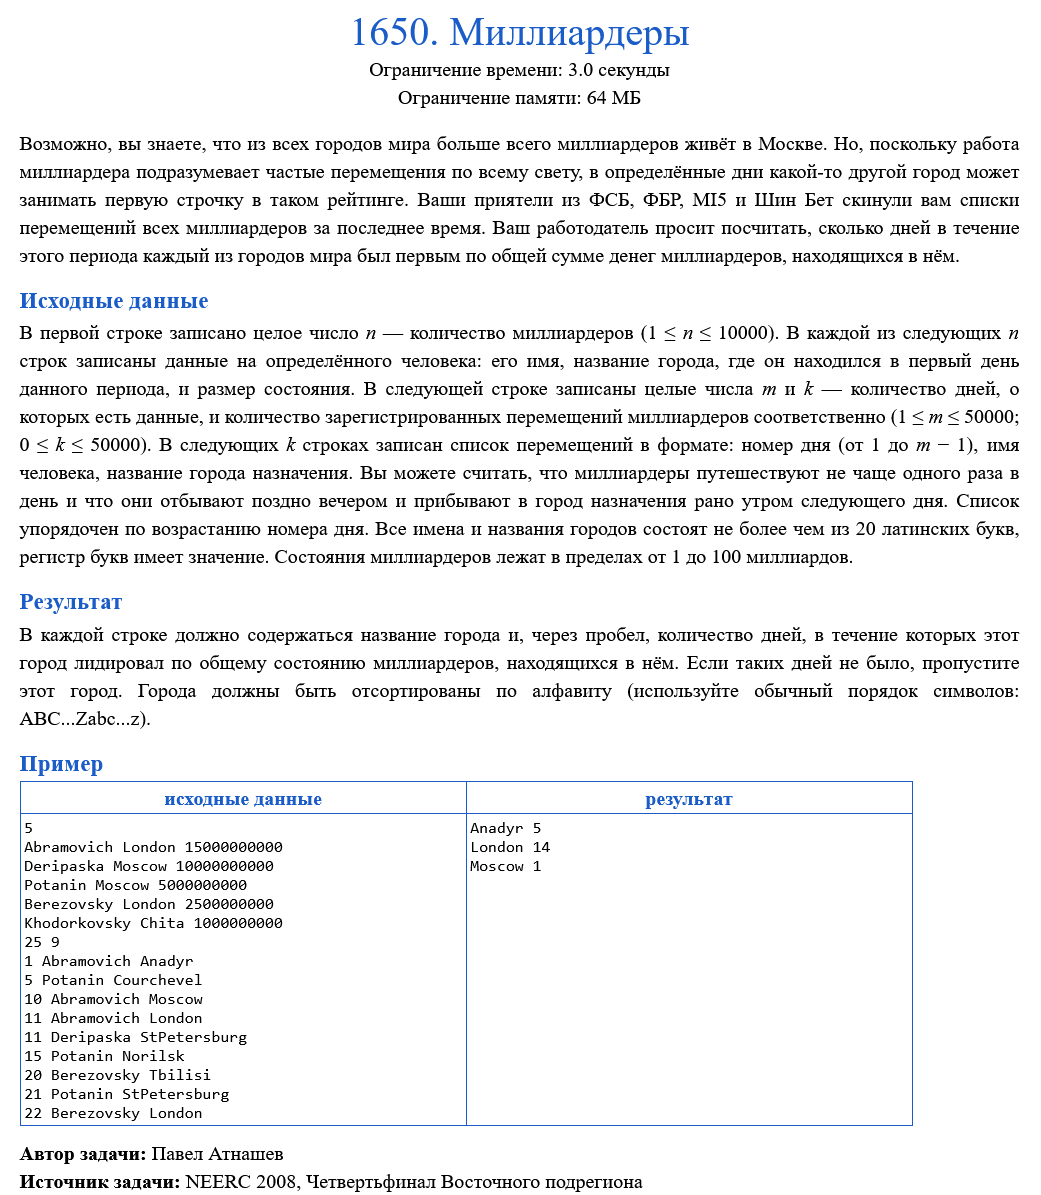
\includegraphics[width=0.9\linewidth]{pic/task_1650.png}}
\caption{Условие задачи 1650.}
\end{figure}

\subsection{Краткое описание алгоритма}
\textbf{1. Входные данные:} в первой строке записано целое число $n$ — количество миллиардеров $(1 \leq n \leq 10000)$. В каждой из следующих $n$ строк записаны данные на определённого человека: его имя, название города, где он находился в первый день данного периода, и размер состояния. \\

В следующей строке записаны целые числа $m$ и $k$ — количество дней, о которых есть данные, и количество зарегистрированных перемещений миллиардеров соответственно $(1 \leq m \leq 50000; 0 \leq k \leq 50000)$. В следующих $k$ строках записан список перемещений в формате: номер дня (от $1$ до $m - 1$), имя человека, название города назначения.\\

 Вы можете считать, что миллиардеры путешествуют не чаще одного раза в день и что они отбывают поздно вечером и прибывают в город назначения рано утром следующего дня. Список упорядочен по возрастанию номера дня. Все имена и названия городов состоят не более чем из 20 латинских букв, регистр букв имеет значение. Состояния миллиардеров лежат в пределах от 1 до 100 миллиардов \\

\textbf{2.}  Создадим структуру, в которой будут находиться отсортированные по неубыванию множество городов, в котором будем хранить актуальное состояние каждого из городов, в случае перелета миллиардера сумма города изменяется, соответственно заново сортируется структура;\\

\textbf{3.}  создадим еще одну структуру данных, в которой будем хранить имя миллиардера и информацию о городе, в котором он находится. Для этого будем использовать \textit{словарь} (или \textit{map}): ключ -- имя миллиардера, значение -- структура, в которой хранится информация о количестве денег и о длительности их нахождения в нем;\\

\textbf{4.} весь алгоритм работает за $O(n \cdot \ln n)$\\

\textbf{5. Выходные данные:} в каждой строке должно содержаться название города и, через пробел, количество дней, в течение которых этот город лидировал по общему состоянию миллиардеров, находящихся в нём. Если таких дней не было, пропустите этот город. Города должны быть отсортированы по алфавиту (используйте обычный порядок символов: ABC...Zabc...z). 

\subsection{Листинг}

\begin{center}
\begin{lstlisting}[label=some-code,caption={Исходный код для 1650}]
#include <iostream>


\end{lstlisting}
\end{center}

\subsection{Результат}
%\begin{figure}[h!]
%\center{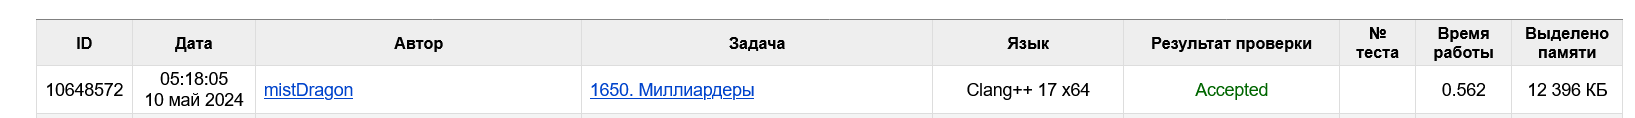
\includegraphics[width=0.9\linewidth]{pic/screen_1650.png}}
%\caption{Результат отправки задачи 1650.}
%\end{figure}







\newpage
\section{Задача 1450}

\begin{figure}[h!]
\center{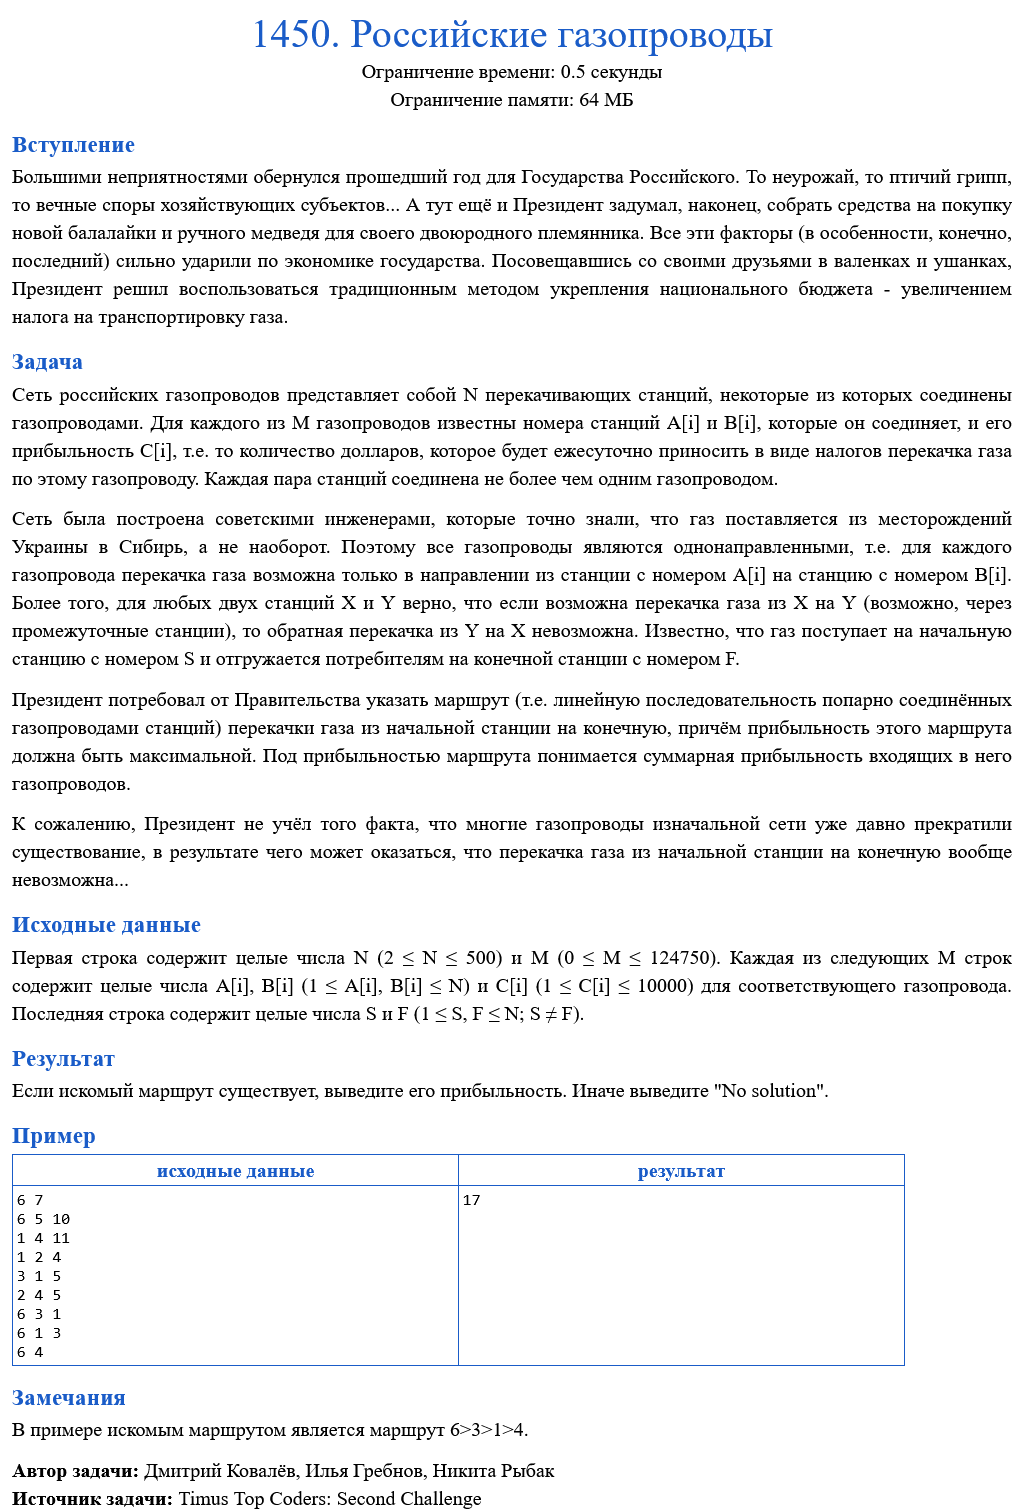
\includegraphics[width=0.8\linewidth]{pic/task_1450.png}}
\caption{Условие задачи 1450.}
\end{figure}

\subsection{Краткое описание алгоритма}
\textbf{1. Входные данные:} \\
\textbf{2.}  \\
\textbf{3.}  \\
\textbf{4.}  \\
\textbf{5. Выходные данные:} 

\subsection{Листинг}

\begin{center}
\begin{lstlisting}[label=some-code,caption={Исходный код для 1450}]
#include <iostream>


\end{lstlisting}
\end{center}

\subsection{Результат}
%\begin{figure}[h!]
%\center{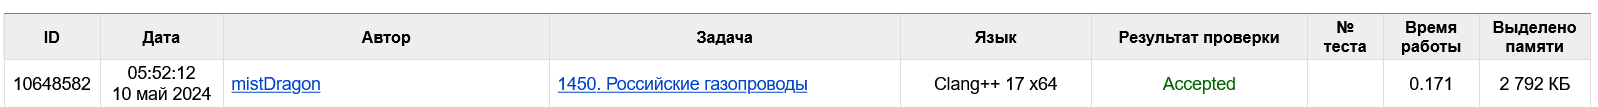
\includegraphics[width=0.9\linewidth]{pic/screen_1450.png}}
%\caption{Результат отправки задачи 1450.}
%\end{figure}









\newpage

\section{Задача 1806}

\begin{figure}[h!]
\center{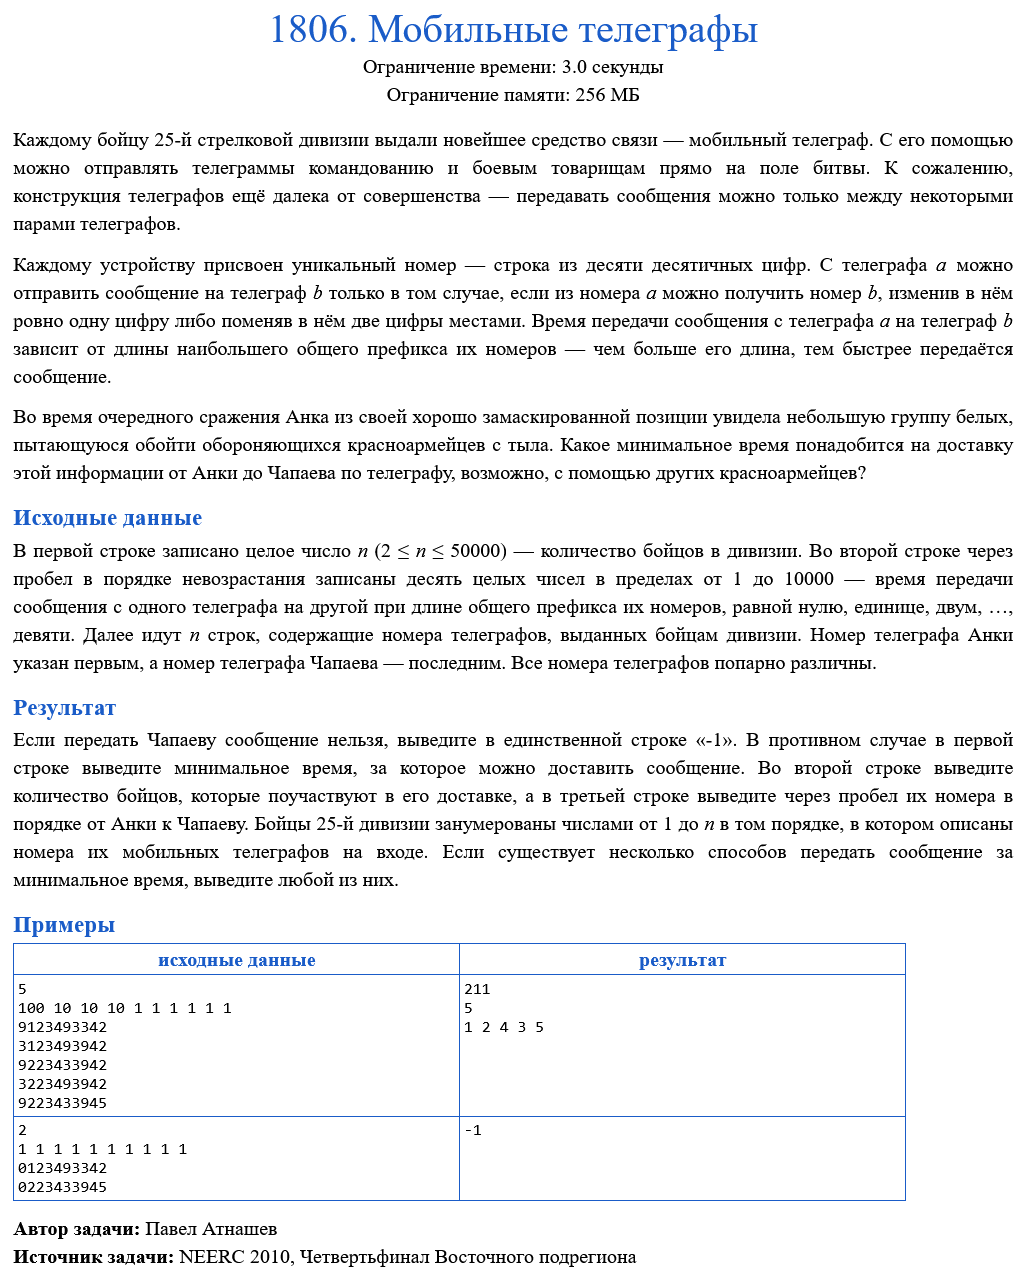
\includegraphics[width=0.9\linewidth]{pic/task_1806.png}}
\caption{Условие задачи 1806.}
\end{figure}

\subsection{Краткое описание алгоритма}
\textbf{1. Входные данные:} \\
\textbf{2.}  \\
\textbf{3.}  \\
\textbf{4.}  \\
\textbf{5. Выходные данные:}

\subsection{Листинг}

\begin{center}
\begin{lstlisting}[label=some-code,caption={Исходный код для 1806}]
#include <iostream>


\end{lstlisting}
\end{center}

\subsection{Результат}
%\begin{figure}[h!]
%\center{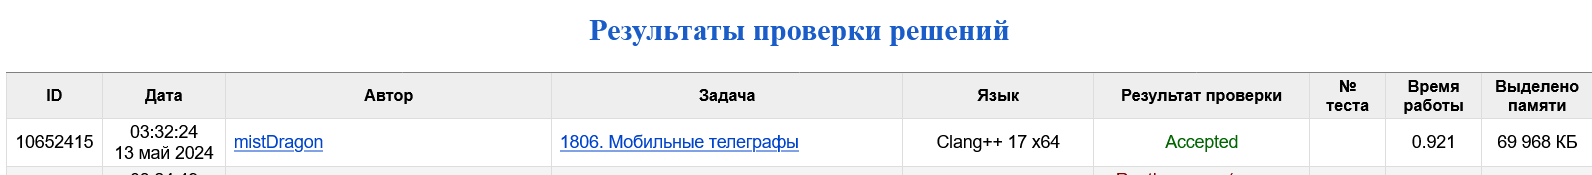
\includegraphics[width=0.9\linewidth]{pic/screen_1806.png}}
%\caption{Результат отправки задачи 1806.}
%\end{figure}



\newpage
\section{Вывод по работе}
В ходе выполнения данной лабораторной работы были реализованы алгоритмы для решения задач $1650$, $1450$ и $1806$. 
\end{document}













